
In this section we consider zero-value seller settings when the buyer's valuation distribution is assumed to be regular. Note that due to \Cref{example:all fair mech:irregular} and \Cref{lem:optimal GFT upper bound:irregular}, when no assumption is made about the valuation distribution, there are instances in which any {\ksfair} mechanism has GFT that is at most half the {\SecondBest}.

By imposing regularity on the buyer's valuation distribution and restricting the seller's value to be deterministically equal to zero, a natural first attempt is to explore whether the {\BiasedRandomOffer} mechanism, as developed in \Cref{cor:biased random offer}, can achieve an improved GFT approximation ratio strictly greater than $\frac{1}{2}$. However, the following example, along with its corresponding lemma, demonstrates the failure of the {\BiasedRandomOffer} to achieve a better GFT approximation.

\begin{example}
\label{example:BROM:regular}
Fix any $\constantH \geq 1$. The buyer has a regular valuation distribution $\buyerdist$, which has support $[0, \constantH]$ and cumulative density function $\buyercdf(\val) = \frac{(\constantH - 1)\cdot \val}{(\constantH - 1)\cdot \val + \constantH}$ for $\val \in[0,\constantH]$ and $\buyercdf(\val) = 1$ for $\val \in(\constantH, \infty)$.
(Namely, there is an atom at $\constantH$ with probability mass of $\frac{1}{\constantH}$.)
The seller has a deterministic value of 0.
See \Cref{fig:BROM:regular} for an illustration.
\end{example}


\begin{restatable}{lemma}{lemBROMregular}
\label{lem:BROM:regular} 
    Fix any $\eps > 0$. In \Cref{example:BROM:regular} with sufficiently large $\constantH$ (as a function of $\eps$), the {\ksfair} {\BiasedRandomOffer} $\mech$ (from \Cref{cor:biased random offer}) obtains less than $(\frac{1}{2} + \eps)$ of the {\SecondBest} $\OPTSB$, i.e., $\GFT{\mech} < (\frac{1}{2} + \eps)\cdot \OPTSB$.
\end{restatable}
\begin{proof}
    In \Cref{example:BROM:regular}, the {\SecondBest} $\OPTSB = \expect[\val]{\val} = (1 - o_{}(1))\cdot \ln\constantH$. The {\ksfair} {\BiasedRandomOffer} $\mech$ is exactly the (unbiased) {\RandomOffer}. Consequently, the GFT of the {\BiasedRandomOffer} $\mech$ is $\GFT{\mech} = (\frac{1}{2} + o_{}(1))\cdot \ln\constantH$. This completes the proof as desired. 
\end{proof}

\Cref{lem:BROM:regular} shows that to obtain a larger fraction of GFT by a {\ksfair} mechanism we cannot use to the {\BiasedRandomOffer}, so next we consider alternative mechanisms. While \Cref{lem:optimal GFT upper bound:irregular} showed that the {\FixPrice} cannot obtain good GFT approximation for general buyer distributions, we move to study it when the distribution is regular. For the setting of \Cref{example:BROM:regular} it can be verified that there exists a particular price $\fprice\in(0, \constantH)$ such that the {\FixPrice} with trading price $\fprice$ is {\ksfair}. To see this, note that for this example, in the {\FixPrice}, as trading price $\price$ increases, the buyer's ex ante utility is continuous and strictly decreasing, while the seller's ex ante utility is continuous and strictly increasing up to the monopoly reserve $\optreserve = \constantH$ (since the buyer's valuation distribution is regular and thus revenue curve is concave). Moreover, at the two extreme cases where price $\price = 0, \constantH$, two traders' ex ante utilities become zero and their benchmarks $\sellerbenchmark, \buyerbenchmark$, respectively. Hence, the existence of {\ksfair} trading price $\fprice\in(0, \constantH)$ is guaranteed by the intermediate value theorem. Finally, for this example, by simple numerical calculation, it can be checked that the GFT approximation of the {\FixPrice} with trading price $\fprice$ is also large. For example, with $\constantH = 25$, the GFT approximation is $\fixedPriceGFTPercentageUBRegular$. (Analytical expression can be found in Eqn.~\eqref{eq:BROM:regular:fair price} and \eqref{eq:BROM:regular:fair price GFT approx}.) 
Also see \Cref{fig:BROM:regular} for an illustration.

As the main result of this subsection, we extend the above observation regarding \Cref{example:BROM:regular} to general zero-value seller instances where the buyer has a regular valuation distribution.\footnote{{We remind that when no assumption (such as regularity) is made for the buyer's valuation distribution, even if the seller is zero-value, any {\ksfair} {\FixPrice} can only achieve $\eps$ fraction of the {\SecondBest} $\OPTSB$ for every $\eps > 0$ (\Cref{lem:optimal GFT upper bound:irregular}).}} Although arguing the existence of such a {\ksfair} {\FixPrice} is relatively easy due to the intermediate value theorem, proving its almost-tight GFT approximation is \emph{technically highly non-trivial}. 

\begin{figure}
    \centering
    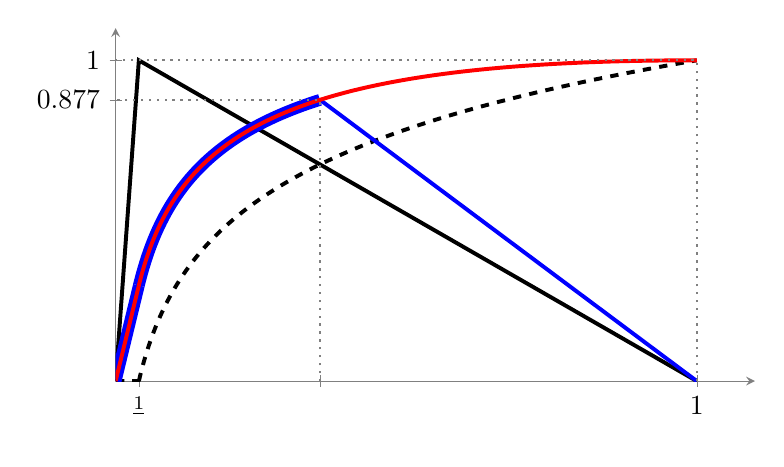
\begin{tikzpicture}[scale=1, transform shape]
\begin{axis}[
axis line style=gray,
axis lines=middle,
xlabel = $\quant$,
xtick={0, 0.04, 0.35168, 1},
ytick={0, 0.8767514, 1},
xticklabels={0, $\frac{1}{\constantH}$, $\fquant$, 1},
yticklabels={0, $0.877$, $1$},
xmin=0,xmax=1.1,ymin=-0.0,ymax=1.1,
width=0.8\textwidth,
height=0.5\textwidth,
samples=500]

\addplot[black!100!white, line width=0.5mm] (0, 0) -- (0.04, 1) -- (1, 0);

\addplot[domain=0:0.04, dashed, line width=0.5mm] (x, {0});
% \addplot[domain=0.04:1, red, line width=0.5mm] (x, {(1 + 25 / 24 * (ln(x) + ln(25) - x + 0.04) - 25 / 24 * (1 - x) / 3.3529956509});
\addplot[domain=0.04:1, dashed, line width=0.5mm] (x, {(1 + 25 / 24 * (ln(x) + ln(25) - x + 0.04) - 25 / 24 * (1 - x)) / 3.3529956509});


\addplot[blue, line width=1.5mm] (0, 0) -- (0.04, 0.2982407);
\addplot[domain=0.04:0.35168, blue, line width=1.5mm] (x, {(1 + 25 / 24 * (ln(x) + ln(25) - x + 0.04)) / 3.3529956509});
\addplot[blue, line width=0.5mm] (0.35168, 0.8767514) -- (1, 0);

\addplot[red, line width=0.5mm] (0, 0) -- (0.04, 0.2982407);
\addplot[domain=0.04:1, red, line width=0.5mm] (x, {(1 + 25 / 24 * (ln(x) + ln(25) - x + 0.04)) / 3.3529956509});



\addplot[dotted, gray, line width=0.3mm] (0.35168, 0) -- (0.35168, 0.8767514) -- (0, 0.8767514);

\addplot[dotted, gray, line width=0.3mm] (1, 0) -- (1, 1) -- (0, 1);



\end{axis}

\end{tikzpicture}
    \caption{Graphical illustration of \Cref{example:BROM:regular} when $\constantH = 25$. The x-axis is quantile $\quant$. 
    The black solid line is the revenue curve of the buyer.
    Consider {\FixPrice} $\mech$ with trading price $\price = \val(\quant)$ for every quantile $\quant$. The black solid (resp.\ dashed) curve also represents   ${\sellerexanteutil(\mech)}/{\sellerbenchmark}$ (resp.\ ${\buyerexanteutil(\mech)}/{\buyerbenchmark}$) for the seller (resp.\ buyer). The red curve is the GFT approximation ratio ${\GFT{\mech}}/{\OPTSB}$. 
    A {\ksfair} {\FixPrice} is achieved at trading price $\fprice = \val(\fquant)$ with GFT approximation ratio of $0.877$ (when $\constantH = 25$).
    Finally, the blue curve is used in the proof of the negative result in \Cref{lem:GFT UB:regular buyer}.}
    \label{fig:BROM:regular}
\end{figure}

\begin{restatable}{theorem}{thmGFTregularbuyer}
\label{thm:improved GFT:regular buyer}
    For every bilateral trade instance of a zero-value seller and a buyer with a regular valuation distribution $\buyerdist$, there exists price $\fprice$ smaller than the smallest monopoly reserve $\optreserve$ for distribution $\buyerdist$, such that the {\FixPrice} with trading price $\fprice$ is {\ksfair} and its GFT is at least $\calC$ fraction of the {\SecondBest} $\OPTSB$. Here $\calC$ is the solution to minimization program~\ref{program:GFT:regular buyer},
    and we observe that 
    $\calC\geq \fixedPriceGFTPercentageRegular$ by a numerical computation.

    Moreover, there exists an instance of a zero-value seller and a  buyer with a regular valuation distribution, in which any BIC, IIR, ex ante WBB mechanism that is {\ksfair} has GFT that is less than  $\fixedPriceGFTPercentageUBRegular$ of the {\SecondBest} $\OPTSB$.
\end{restatable}

\Cref{thm:improved GFT:regular buyer} follows directly from two technical lemmas (\Cref{lem:GFT program:regular buyer,lem:GFT UB:regular buyer}) which establish the positive and negative results in the theorem statement respectively. The technical overview of our argument are given under each lemma.


\subsubsection{GFT Approximation by KS-Fair {\FixPrice}}
We characterize the GFT approximation of a {\ksfair} {\FixPrice} as follows.
\begin{figure}
    \centering
    \begin{tikzpicture}[scale=1, transform shape]
\begin{axis}[
axis line style=gray,
axis lines=middle,
% xlabel = $\quant$,
% ylabel = $\revcurve$,
xtick={0, 0.5, 0.625, 0.75, 1},
ytick={0, 0.25, 0.75, 1},
xticklabels={0, $\optquant$, $\quant_0$, $\quant$,  1},
yticklabels={0, $\val_0$, $\alpha$, $1$},
xmin=0,xmax=1.1,ymin=-0.0,ymax=1.5,
width=0.8\textwidth,
height=0.5\textwidth,
samples=500]

% \fill[blue!20] (0,0) -- (0.642857, 0.229591877551) -- (0.725, 0.199375) -- cycle;



\addplot[domain=0:0.625, red, line width=0.5mm] (x, {1});
\addplot[domain=0.625:1, red, line width=0.5mm] (x, {-2*(x-0.75)+0.75});
\addplot[dotted, gray, line width=0.3mm] (0.625, 0) -- (0.625, 1);

\addplot[line width=0.5mm, blue] (0, 0) -- (0.5, 1) -- (0.75, 0.75) -- (1, 0);

\addplot[domain=0:1, black!100!white, line width=0.5mm] (x, {x * (1-x) / 0.25}); 

\addplot[dotted, gray, line width=0.3mm] (1, 0) -- (1, 0.25) -- (0, 0.25);


% \addplot[line width=0.5mm, dashed] (0, 0) -- (0.6, 1.2);
\addplot[dotted, gray, line width=0.3mm] (0.5, 0) -- (0.5, 1) -- (0, 1);
% \draw (0.63, 1.25) node {$\optreserve$};
\addplot[dotted, gray, line width=0.3mm] (0.5, 1) -- (1, 1);

% \addplot[line width=0.5mm, dashed] (0, 0) -- (0.9, 0.9);
\addplot[dotted, gray, line width=0.3mm] (0.75, 0) -- (0.75, 0.75) -- (0, 0.75);
% \draw (0.93, 0.92) node {$\price$};

% \addplot[line width=0.5mm, dashed] (0, 0) -- (0.7, 0.25);

% \addplot[dotted, gray, line width=0.3mm] (0.725, 0) -- (0.725, 0.199375);% -- (0, 0.199375);

% \addplot[dotted, gray, line width=0.3mm] (0.642857, 0.176785675) -- (0, 0.176785675);

% \addplot[dotted, gray, line width=0.3mm] (0.642857, 0) -- (0.642857, 0.229591877551) -- (0, 0.229591877551);



\draw[decorate,decoration={brace,amplitude=8pt}] (0.0,1.3) -- (0.5,1.3) node[midway,above=6pt] {$H$/{{\color{red}$\HOverBar$}}/{{\color{blue}$\HUnderBar$}}};
\draw[decorate,decoration={brace,amplitude=8pt}] (0.5,1.3) -- (0.75,1.3) node[midway,above=6pt] {$M$/{{\color{red}$\MOverBar$}}/{{\color{blue}$\MUnderBar$}}};
\draw[decorate,decoration={brace,amplitude=8pt}] (0.75,1.3) -- (1,1.3) node[midway,above=6pt] {$L$/{{\color{red}$\LOverBar$}}/{{\color{blue}$\LUnderBar$}}};
\addplot[dotted, gray, line width=0.3mm] (0.5, 1) -- (0.5, 1.3);
\addplot[dotted, gray, line width=0.3mm] (0.75, 0.75) -- (0.75, 1.3);
\addplot[dotted, gray, line width=0.3mm] (1, 0.25) -- (1, 1.3);

\end{axis}

\end{tikzpicture}
    \caption{Graphical illustration of the analysis for \Cref{lem:GFT program:regular buyer}. The black curve is the concave revenue curve $\revcurve$ of the buyer. The red and blue revenue curves $\revcurve_1, \revcurve_2$ (defined in the analysis) sandwich the original revenue curve $\revcurve$.}
    \label{fig:GFT program:regular buyer}
\end{figure}
\begin{lemma}
\label{lem:GFT program:regular buyer}
    For every bilateral trade instance of a zero-value seller and buyer with regular valuation distribution $\buyerdist$, there exists price $\fprice$ smaller than the smallest monopoly reserve $\optreserve$ for distribution $\buyerdist$, such that the {\FixPrice} with trading price $\fprice$ is {\ksfair} and its GFT is at least $\calC$ fraction of the {\SecondBest} $\OPTSB$. Here $\calC$ is the solution to the following program~\ref{program:GFT:regular buyer}:
    \begin{align}
    \label{program:GFT:regular buyer}
    \tag{$\mathcal{P}_{\mathrm{REG}}$}
    \arraycolsep=5.4pt\def\arraystretch{1}
        \begin{array}{llll}
          \calC \triangleq~~&\min\limits_{\optquant, H}
          ~\max\limits_{\revratio}
          ~\min\limits_{\substack{\quant, \val_0, M, L}}   & 
          \displaystyle\exanteutilratio + \frac{\exanteutilratio}{H + M + L} &
          \vspace{10pt}
          \\
          \vspace{10pt}
          &\text{s.t.}
          & \optquant\in[0, 1]~,  & 
          \\
          \vspace{10pt}
          && \revratio\in(0, 1)~,  & 
          \\ 
          \vspace{10pt}
          && \quant\in \left[\optquant + (1 - \revratio)(1 - \optquant), 1\right]~,  & 
          \\
          \vspace{10pt}
          && \val_0\in \left[0, 1 - \displaystyle\frac{1 - \revratio}{\quant - \optquant}(1 - \optquant)\right]~,  & 
          \\
          \vspace{10pt}
          && H\in\left[\HUnderBar, \HOverBar\right]~, 
          M\in\left[\MUnderBar, \MOverBar\right]~,
          L\in\left[\LUnderBar, \LOverBar\right]~,& 
        \end{array}
    \end{align}
    where $\exanteutilratio$, $\quant_0$, $\HUnderBar, \HOverBar, \MUnderBar, \MOverBar, \LUnderBar, \LOverBar$ are auxiliary variables constructed as 
    \begin{align*}
        \exanteutilratio &\triangleq  \displaystyle
        \revratio - \plus{\frac{H + M + L}{H + M + L + 1}\left(\revratio - \frac{H + M - \revratio}{H + M + L}\right)}~,
        \\
        \quant_0 &\triangleq 1 - \frac{(1 - \val_0)(1 - q)}{\revratio - \val_0}~,
        \\
        \HUnderBar &\triangleq 1~, \HOverBar \triangleq \infty~, 
        \\
        \MUnderBar &\triangleq \ln\left(\frac{q}{\optquant}\right)\left(1 + \frac{1 - \revratio}{q - \optquant}\optquant\right) - 1 + \revratio ~,
        \\
        \MOverBar &\triangleq  \ln\left(\frac{\quant_0}{\optquant}\right) 
        +
        \ln\left(\frac{q}{\quant_0}\right)\left(\val_0 + \frac{\revratio - \val_0}{1 - q}\right) 
        -
        \frac{q - \quant_0}{1 - q}(\revratio - \val_0)~,
        \\
        \LUnderBar &\triangleq \frac{\revratio}{1 - \quant}\ln\left(\frac{1}{\quant}\right)~,
        % \\
        \LOverBar \triangleq \ln\left(\frac{1}{q}\right)\left(\val_0 + \frac{\revratio - \val_0}{1 - q}\right) - \revratio + \val_0~.
    \end{align*}
    By a numerical computation (see \Cref{apx:numerical evaluation:regular buyer}), we observe that 
    $\calC\geq \fixedPriceGFTPercentageRegular$.
\end{lemma}

\xhdr{Proof overview of \Cref{lem:GFT program:regular buyer}.} We first explain the idea of proving the lemma above and the optimization program in its statement. As we explained before, to obtain an GFT approximation better than $\frac{1}{2}$, we cannot compare the GFT with $\sellerbenchmark + \buyerbenchmark$, since it may be twice larger than the {\SecondBest}.\footnote{Since the seller has zero value, the first and {\SecondBest}s both equal to the expected value of the buyer, i.e., $\OPTFB = \OPTSB = \expect[\val]{\val}$.} Hence, unlike the proof of \Cref{thm:blackbox reduction} in the previous section, our analysis of \Cref{lem:GFT program:regular buyer} aims to directly compare the GFT of a {\ksfair} {\FixPrice} with the {\SecondBest}. Loosely speaking, {for a given regular distribution} we establish a lower bound on the GFT approximation. We then search over all regular distributions and argue that the worst regular distribution that minimizes the established GFT lower bound belongs to a distribution subclass, whose revenue curve can be characterized by finite many parameters (i.e., variables in the optimization program in the statement of \Cref{lem:GFT program:regular buyer}, also see \Cref{fig:GFT program:regular buyer}). For this distribution subclass, we lower bound its GFT approximation as program~\ref{program:GFT:regular buyer}.

Reducing the class of regular distributions to a subclass with finitely many parameters is a common technique for deriving approximation bounds in the mechanism design literature \citep[e.g.,][]{AHNPY-18, JLQTX-19, FHL-21, JL-23}. However, most prior work focuses on revenue approximation and allows consideration of a class of mechanisms (e.g., anonymous pricing with all possible prices). This makes it relatively easy to argue that the approximation ratio depends on a \emph{small set} of parameters (e.g., monopoly quantile, monopoly price) of the revenue curve. In contrast, our analysis requires studying both revenue and GFT (expected value). Furthermore, we focus on a single mechanism ({\ksfair} {\FixPrice}). Hence, both the GFT benchmark and the GFT of our mechanism are highly sensitive to the \emph{entire} revenue curve.

To overcome this challenge, our technical lemma (\Cref{lem:GFT program:regular buyer}) develops a three-step argument. We first consider a (possibly not {\ksfair}) {\FixPrice} whose trading price $\price$ is selected based on a \emph{small set} of parameters of the revenue curve. In particular, depending on the monopoly quantile $\optquant$ and the expected value $H = \expect[\val]{\val\cdot \indicator{\val \geq \optreserve}}$ above the monopoly reserve $\optreserve$, we select a constant $\revratio\in(0, 1)$ and let $\price$ be the trading price smaller than the monopoly reserve such that by posting price $\price$, the seller's ex ante utility (revenue) is $\revratio$ fraction of her benchmark (monopoly revenue) $\sellerbenchmark$, i.e., $\price\cdot(1 - \buyercdf(\price)) = \revratio\cdot \sellerbenchmark$. Our second step is conceptually similar to our previous black-box reduction (\Cref{thm:blackbox reduction}). In particular, we argue that depending on buyer's ex ante utility under trading price $\price$, we can decrease (or increase) this price to obtain a {\ksfair} trading price $\fprice$. This step allows us to lower bound the GFT approximation of a {\ksfair} {\FixPrice} mechanism with trading price $\fprice$ as a \emph{function of the price $\price$ chosen in the first step}. Finally, since this GFT lower bound depends on the choice of $\price$ determined in the first step, we formulate the problem of selecting the optimal price $\price$ (to maximize the GFT approximation lower bound) as a two-player zero-sum game. In this game, the ``min player'' (adversary) selects the revenue curve (represented by finitely many quantities on the revenue curve), while the ``max player'' (ourselves) selects the price $\price$. The game's payoff is the GFT approximation lower bound derived in the second step. Finally, we numerically solve this two-player zero-sum game and obtain $\fixedPriceGFTPercentageRegular$ stated in the lemma. 


\begin{proof}[Proof of \Cref{lem:GFT program:regular buyer}]
    Let $\revcurve$ be the revenue curve of the buyer and $\optquant\in \argmax_{\quant}\revcurve(\quant)$ be the monopoly quantile. If there exist multiple monopoly quantiles, we let $\optquant$ be the largest one. Without loss of generality, we normalize the monopoly revenue to be equal to one, i.e., $\revcurve(\optquant) = 1$ and thus monopoly reserve $\optreserve = \frac{1}{\optquant}$. Since the buyer's valuation distribution is regular, revenue curve $\revcurve$ is concave (\Cref{lem:concave revenue curve}).
    
    \xhdr{Step 0- Introducing necessary notations.} We introduce $\revratio\in(0, 1)$ as a constant whose value will be pined down at the end of this analysis. Given constant $\revratio$, let $\quant\in[\optquant, 1]$ be the largest quantile such that $\revcurve(\quant) \geq \revratio$. Moreover, let $\val_0 \triangleq \revcurve(\quant) + (1-\quant)\cdot \revcurve'(\quant)$ and $\quant_0 \triangleq \quant + (1 - \revratio) / \revcurve'(\quant)$. Finally, we also define 
    \begin{align*}
        H &\triangleq \expect[\val]{\val\cdot \indicator{\val \geq \optreserve}},
        \;\;
        M \triangleq \expect[\val]{\val\cdot \indicator{\revratio/\quant \leq \val < \optreserve}},
        \;\;
        L \triangleq \expect[\val]{\val\cdot \indicator{ \val < \revratio/\quant}}
    \end{align*}
    which partition the {\SecondBest} into three pieces, i.e., $\OPTSB = \expect[\val]{\val} = H + M + L$. All notations are illustrated in \Cref{fig:GFT program:regular buyer}.

    \xhdr{Step 1- Characterizing of a (possibly) not {\ksfair} {\FixPrice}.}
    First, we consider a (possibly not {\ksfair}) {\FixPrice} ({$\FPM_{\price}$}) with trading price $\price = \frac{\revratio}{\quant}$:
    \begin{itemize}
        \item For the seller, her ex ante utility (aka., revenue) is $\sellerexanteutil(\FPM_{\price}) = \price\cdot (1 - \buyercdf(\price)) = \price\cdot \quant = \revratio$. Since her benchmark $\sellerbenchmark$ (aka., monopoly revenue) is normalized to one, her ex ante utility is an $\alpha$ fraction of her benchmark $\sellerbenchmark$.
        \item For the buyer, her ex ante utility can be computed as 
        \begin{align*}
            \buyerexanteutil(\FPM_{\price}) &= 
            \expect[\val]{\plus{\val - \price}} = 
            H + M - \revratio
        \end{align*}
        Meanwhile, the buyer's benchmark $\buyerbenchmark$ is 
        \begin{align*}
            \buyerbenchmark = H + M + L
        \end{align*}
    \end{itemize}
    Putting the two pieces together, we conclude that in this (possibly not {\ksfair}) {\FixPrice} ({$\FPM_{\price}$}), both traders' ex ante utilities satisfy
    \begin{align*}
        \frac{\sellerexanteutil(\FPM_{\price})}{\sellerbenchmark} = \revratio
        \;\;
        \mbox{and}
        \;\;
        \frac{\buyerexanteutil(\FPM_{\price})}{\buyerbenchmark} = \frac{H + M - \revratio}{H + M + L}
    \end{align*}
    
    \xhdr{Step 2- Characterizing of {\ksfair} {\FixPrice}.} Define auxiliary notation $\exanteutilratio\in[0, 1]$ as 
    \begin{align*}
        \exanteutilratio \triangleq \displaystyle
        \revratio - \plus{\frac{H + M + L}{H + M + L + 1}\left(\revratio - \frac{H + M - \revratio}{H + M + L}\right)}
    \end{align*}
    We next show that there exists price $\fprice\in[0,\optreserve]$ such that the {\FixPrice} with trading price $\fprice$ is {\ksfair} and both traders' ex ante utilities are at least $\exanteutilratio$ fraction of their benchmarks $\sellerbenchmark,\buyerbenchmark$, respectively. To see this, consider the following two cases separately.
    \begin{itemize}
        \item Suppose that $\revratio < \frac{H + M - \revratio}{H + M + L}$ and thus $\exanteutilratio = \revratio$. In this case, by increasing trading price $\price$ in the {\FixPrice}, the seller's ex ante utility increases continuously (due to the concavity of revenue curve $\revcurve$) and the buyer's ex ante utility decreases continuously. Invoking the intermediate value theorem, there exists price $\fprice \in (\price, \optreserve)$ such that both traders' ex ante utilities is at least $\exanteutilratio$ fraction of their benchmarks $\sellerbenchmark,\buyerbenchmark$, respectively.
        \item Suppose that $\revratio \geq \frac{H + M - \revratio}{H + M + L}$ and thus $\exanteutilratio = \revratio - {\frac{H + M + L}{H + M + L + 1}\left(\revratio - \frac{H + M - \revratio}{H + M + L}\right)}$. In this case, let $\Delta \triangleq {\frac{H + M + L}{H + M + L + 1}\left(\revratio - \frac{H + M - \revratio}{H + M + L}\right)}\geq 0$. By decreases trading price $\price$ in the {\FixPrice}, the seller's ex ante utility decreases continuously (due to the concavity of revenue curve $\revcurve$). Let $\price\primed < \price$ be the trading price such that the seller's ex ante   utility (aka., revenue) is equal to $\revratio - \Delta$. Under trading price $\price\primed$, the buyer's ex ante utility is at least $H + M - \revratio + \Delta$. (To see this, note that by decreasing trading price from $\price$ to $\price\primed$, the GFT weakly increases and the seller's ex ante utility decreases by $\Delta$. Thus, the buyer's ex ante utility increases by at least $\Delta$.) Due to the definition of $\Delta$, two traders' ex ante utilities in the {\FixPrice} ($\FPM_{\price\primed}$) with trading price $\price\primed$ satisfy
        \begin{align*}
            \frac{\sellerexanteutil(\FPM_{\price\primed})}{\sellerbenchmark} = \revratio - \Delta = \frac{H + M - \revratio + \Delta}{H + M + L}
            \leq 
            \frac{\buyerexanteutil(\FPM_{\price\primed})}{\buyerbenchmark}
        \end{align*}
        If the inequality above holds with equality, the {\FixPrice} with trading price $\price\primed$ is {\ksfair} and both traders' ex ante utilities are at least $\exanteutilratio$ fraction of their benchmarks $\sellerbenchmark,\buyerbenchmark$, respectively. Otherwise, we can invoke argument in the previous case.
    \end{itemize}
    Summarizing the analysis above, the GFT-approximation of the {\ksfair} {\FixPrice} ($\FPM_{\fprice}$) with trading price $\fprice$ can be computed as 
    \begin{align*}
        \frac{\GFT{\FPM_{\fprice}}}{\OPTSB}
        \geq
        \frac{\exanteutilratio \cdot (\sellerbenchmark + \buyerbenchmark)}{\expect[\val]{\val}}
        =
        \exanteutilratio + \frac{\exanteutilratio}{H + M + L}
    \end{align*}

    \xhdr{Step 3- Formulating GFT approximation as two-player game.} Putting all the pieces together, the optimization program in the lemma statement can be viewed as a two-player zero-sum game between a min player (adversary) and a max player (ourself as GFT-approximation prover). The payoff in this game is the GFT approximation lower bound $\exanteutilratio + \frac{\exanteutilratio}{H + M + L}$ shown above. As a reminder, quantities $\exanteutilratio, H, M, L$ depend on both the buyer's valuation distribution and constant $\revratio$ used in the analysis. The min player chooses the worst regular distribution (equivalently, concave revenue curve) of the buyer, and the max player chooses constant $\revratio$. Importantly, the choice of constant $\revratio$ can depend on the buyer's valuation distribution. To capture this, we formulate this two-player zero-sum game in three stages: 
    \begin{itemize}
        \item (Stage 1) The min player (adversary) chooses monopoly quantile $\optquant$ and $H$.
        \item (Stage 2) The max player (ourself as GFT-approximation prover) chooses constant $\revratio$ for the analysis.
        \item (Stage 3) The min player (adversary) chooses $\val_0, \quant, M, L$.
    \end{itemize}
    It remains to verify that all constraints in the optimization program capture the feasibility condition for the both min player and max player's actions. We next verify the non-trivial constraints individually. 
    \begin{itemize}
        \item (Lower bound for quantile $\quant$) Recall that $\quant\in[\optquant, 1]$ is the largest quantile such that $\revcurve(\quant) \geq \revratio$. 
        The concavity of revenue curve $\revcurve$ implies that $\revcurve(\quant) \geq \frac{1-\quant}{1-\optquant}\revcurve(\optquant)$. Since $\revcurve(\quant) = \revratio$ and $\revcurve(\optquant) = 1$, we obtain $\quant\geq \optquant + (1 - \revratio)(1 - \optquant)$ as stated in the constraint.
        \item (Upper bound for value $\val_0$) Recall that $\val_0 \triangleq \revcurve(\quant) + (1-\quant)\cdot \revcurve'(\quant)$. The concavity of revenue curve $\revcurve$ implies that $\revcurve'(\quant) \leq \frac{\revcurve(\quant) - \revcurve(\optquant)}{\quant - \optquant} = \frac{\revratio - 1}{\quant - \optquant}$. After rearranging, we obtain $\val_0 \leq 1 - \frac{1 - \revratio}{\quant - \optquant}(1 - \optquant)$ as stated in the constraint.
        \item (Bounds for truncated GFT $L$) Recall that $L \triangleq \expect[\val]{\val\cdot \indicator{ \val < \revratio/\quant}}$. The concavity of the revenue curve implies that for every quantile $\quant\primed \in [\quant, 1]$,
        \begin{align*}
            \frac{1 - \quant\primed}{1 - \quant}\cdot \revcurve(\quant)
            \leq 
            \revcurve(\quant\primed) 
            \leq
            \frac{1 - \quant\primed}{1 - \quant}
            \cdot (\revcurve(\quant) - \val_0)
            +
            \val_0
        \end{align*}
        where both inequalities bind at $\quant\primed = \quant$. The left-hand side and right-hand side can be viewed as two revenue curves $\revcurve_1, \revcurve_2$ that sandwich the original revenue curve $\revcurve$ (see blue and red revenue curves illustrated in \Cref{fig:GFT program:regular buyer}). It can be verified that $\LUnderBar$ and $\LOverBar$ are $\expect[\val]{\val\cdot \indicator{ \val < \revratio/\quant}}$ where the random value $\val$ is realized from valuation distribution induced by those two revenue curves $\revcurve_1, \revcurve_2$, respectively. Invoking \Cref{lem:revenue curve monotonicity}, we obtain $\LUnderBar\leq L \leq \LOverBar$ as stated in the constraint, since these two revenue curves $\revcurve_1, \revcurve_2$ sandwich the original revenue curve $\revcurve$.
        \item (Bounds for truncated GFT $M$) The argument is similar to the argument above for truncated GFT $L$. Recall that $M \triangleq \expect[\val]{\val\cdot \indicator{ \revratio/\quant \leq \val <\optreserve }}$. The concavity of the revenue curve implies that for every quantile $\quant\primed \in [\optquant, \quant]$,
        \begin{align*}
            \frac{\quant\primed - \optquant}{\quant - \optquant}\cdot (\revcurve(\optquant) - \revcurve(\quant)) + \revcurve(\quant)
            \leq 
            \revcurve(\quant\primed) 
            \leq
            \min\left\{ \revcurve(\optquant), 
            \frac{\quant\primed - \optquant}{\quant - \quant_0}\cdot (\revcurve(\optquant) - \revcurve(\quant)) + \revcurve(\quant)
            \right\}
        \end{align*}
        where both inequalities bind at $\quant\primed = \optquant$ and $\quant\primed = \quant$. The left-hand side and right-hand side can be viewed as two revenue curves $\revcurve_1, \revcurve_2$ that sandwich the original revenue curve $\revcurve$ (see blue and red revenue curves illustrated in \Cref{fig:GFT program:regular buyer}). It can be verified that $\MUnderBar$ and $\MOverBar$ are $\expect[\val]{\val\cdot \indicator{ \revratio/\quant \leq \val <\optreserve }}$ where the random value $\val$ is realized from valuation distribution induced by those two revenue curves $\revcurve_1, \revcurve_2$, respectively. Invoking \Cref{lem:revenue curve monotonicity}, we obtain $\MUnderBar\leq M \leq \MOverBar$ as stated in the constraint, since these two revenue curves $\revcurve_1, \revcurve_2$ sandwich the original revenue curve $\revcurve$.
        \item (Bounds for truncated GFT $H$) The argument is similar to the argument above for truncated GFT $L$. Recall that $H \triangleq \expect[\val]{\val\cdot \indicator{\val \geq \optreserve}}$. The concavity of the revenue curve and monopoly revenue $\revcurve(\optreserve) = 1$ imply that for every quantile $\quant\primed \in [0, \optquant]$,
        \begin{align*}
            \frac{\quant\primed}{\optquant}\cdot \revcurve(\optquant)
            \leq 
            \revcurve(\quant\primed) 
            \leq
             \revcurve(\optquant)
        \end{align*}
        where both inequalities bind at $\quant\primed = \optquant$. The left-hand side and right-hand side can be viewed as two revenue curves $\revcurve_1, \revcurve_2$ that sandwich the original revenue curve $\revcurve$ (see blue and red revenue curves illustrated in \Cref{fig:GFT program:regular buyer}). It can be verified that $\HUnderBar$ and $\HOverBar$ are $\expect[\val]{\val\cdot \indicator{  \val \geq\optreserve }}$ where the random value $\val$ is realized from valuation distribution induced by those two revenue curves $\revcurve_1, \revcurve_2$, respectively. Invoking \Cref{lem:revenue curve monotonicity}, we obtain $\HUnderBar\leq H \leq \HOverBar$ as stated in the constraint, since these two revenue curves $\revcurve_1, \revcurve_2$ sandwich the original revenue curve~$\revcurve$.
        \item (Equation for quantile $\quant_0$) Recall that  $\quant_0 \triangleq \quant + (1 - \revratio) / \revcurve'(\quant)$ and $\val_0 \triangleq \revcurve(\quant) + (1-\quant)\cdot \revcurve'(\quant)$. Combining both equations with $\revcurve(\quant) = \revratio$, we obtain $\quant_0 = 1 - \frac{(1 - \val_0)(1 - q)}{\revratio - \val_0}$ as stated in the optimization program.
    \end{itemize}
    Finally, we numerically evaluation the optimization program and obtain $\fixedPriceGFTPercentageRegular$. We present more details of this numerical evaluation in \Cref{apx:numerical evaluation:regular buyer}. This completes the proof of \Cref{lem:GFT program:regular buyer}.
\end{proof}

\begin{lemma}
\label{lem:revenue curve monotonicity}
    Given any two distributions $\buyerdist_1,\buyerdist_2$ and any two value $\val\primed, \val\doubleprimed$ with $\val\primed \leq \val\doubleprimed$. 
    Suppose $1-\buyercdf_1(\val\primed) = 1-\buyercdf_2(\val\primed)\triangleq \quant\primed$ and $1-\buyercdf_1(\val\doubleprimed) = 1-\buyercdf_2(\val\doubleprimed)\triangleq\quant\doubleprimed$. If the induced revenue curves $\revcurve_1,\revcurve_2$ satisfy that for every quantile $\quant \in[\quant\doubleprimed,\quant\primed]$,
    $\revcurve_1(\quant) \leq \revcurve_2(\quant)$,
    then 
    \begin{align*}
        \expect[\val\sim\buyerdist_1]{\val\cdot \indicator{\val\primed \leq \val\leq \val\doubleprimed}}
        \leq 
        \expect[\val\sim\buyerdist_2]{\val\cdot \indicator{\val\primed \leq \val\leq \val\doubleprimed}}
    \end{align*}
\end{lemma}
\begin{proof}
    Since for every quantile $\quant \in[\quant\doubleprimed,\quant\primed]$,
    $\revcurve_1(\quant) \leq \revcurve_2(\quant)$ and the inequality is binding at $\quant = \quant\primed$ and $\quant = \quant\doubleprimed$, it is guaranteed that for every value $\val\in[\val\primed,\val\doubleprimed]$, $\buyercdf_1(\val) \geq \buyercdf_2(\val)$
    and the inequality is binding at $\val = \val\primed$ and $\val = \val\doubleprimed$. This is sufficient to prove the lemma statement:
    \begin{align*}
        &\expect[\val\sim\buyerdist_1]{\val\cdot \indicator{\val\primed \leq \val\leq \val\doubleprimed}} 
        =
        \displaystyle\int_{\val\primed}^{\val\doubleprimed}
        \val\cdot \d \buyercdf_1(\val) 
        \overset{(a)}{=}
        \val\doubleprimed \buyercdf_1(\val\doubleprimed)
        -
        \val\primed\buyercdf_1(\val\primed)
        -
        \displaystyle\int_{\val\primed}^{\val\doubleprimed}
        \buyercdf_1(\val) \cdot \d \val
        \\
        &\qquad\overset{(b)}{\leq}
        \val\doubleprimed \buyercdf_2(\val\doubleprimed)
        -
        \val\primed\buyercdf_2(\val\primed)
        -
        \displaystyle\int_{\val\primed}^{\val\doubleprimed}
        \buyercdf_2(\val) \cdot \d \val
        \overset{(c)}{=}  
        \displaystyle\int_{\val\primed}^{\val\doubleprimed}
        \val\cdot \d \buyercdf_2(\val) 
        =
        \expect[\val\sim\buyerdist_2]{\val\cdot \indicator{\val\primed \leq \val\leq \val\doubleprimed}} 
    \end{align*}
    where equalities~(a) (c) hold due to the integration by parts, and inequality~(b) holds as we argued above. This complete the proof of \Cref{lem:revenue curve monotonicity}.
\end{proof}

\subsubsection{Negative Result for Zero-Value Seller and Buyer with a Regular Distribution}

In this part, we establish the negative result (\Cref{lem:GFT UB:regular buyer}) for a zero-value seller and a buyer with regular valuation distribution by analyzing \Cref{example:BROM:regular}.

\begin{lemma}
    \label{lem:GFT UB:regular buyer}
    In \Cref{example:BROM:regular} with $\constantH = 25$, any BIC, IIR, ex ante WBB mechanism $\mech$ that is {\ksfair} has GFT that is less than $\fixedPriceGFTPercentageUBRegular$ of the {\SecondBest} $\OPTSB$. Here $\fixedPriceGFTPercentageUBRegular$ is the numerical evaluated upper bound of the following expression with $\constantH = 25$:\footnote{The \emph{Lambert $W$ function}, also called the \emph{omega function} or \emph{product logarithm} in mathematics, is the converse relation of the function $y(x) = x\cdot e^x$. The principal branch $x = \LambertFunc(y)$ is the inverse relation when $x \geq -1$.} 
    \begin{align*}
    \frac{\constantH\ln\constantH- (\constantH - 1)\cdot \LambertFunc\left(\frac{\constantH^{\frac{\constantH}{\constantH - 1}}\ln (\constantH)}{\constantH-1}\right)}{\constantH\ln \constantH}\cdot \left(\frac{\constantH}{\constantH - 1}+\frac{1}{\ln\constantH}\right)
    \end{align*}
\end{lemma} 
The main difficulty to prove the lemma above is to establish such a GFT approximation bound for \emph{all} BIC, IIR, ex ante WBB, {\ksfair} mechanisms, which may be more complicated than a {\ksfair} {\FixPrice}. Loosely speaking, we first construct an upper bound of GFT (see \eqref{eq:fixed price mech suffices:regular UB}) for every BIC, IIR, ex ante WBB, and {\ksfair} mechanisms. We then argue that for this example, a {\ksfair} {\FixPrice} (which is DSIC, ex post IR, ex post SBB) optimizes this upper bound among all BIC, IIR, ex ante WBB, but (possibly not {\ksfair}) mechanisms. 


\begin{proof}[Proof of \Cref{lem:GFT UB:regular buyer}]
Fix any BIC, IIR, ex ante WBB mechanism $\mech=(\alloc,\price,\sellerprice)$ that is {\ksfair}.  
Let $\revratio(\mech)$ be the ratio between the buyer's expected payment over the monopoly revenue, and $\residuesurplusratio(\mech)$ be the ratio between the buyer's ex ante utility and her expected value. Namely,
\begin{align*}
    \revratio(\mech) \triangleq  
    \frac{\expect[\val]{\price(\val,0)}}{\sellerbenchmark}
    =
    \frac{\sellerexanteutil(\mech) + \expect[\val]{\price(\val,0) - \sellerprice(\val,0)}}{\sellerbenchmark} 
    \;\;
    \mbox{and}
    \;\;
    \residuesurplusratio(\mech) \triangleq \frac{\buyerexanteutil(\mech)}{\buyerbenchmark}
\end{align*}
Since mechanism $\mech$ is ex ante WBB and {\ksfair}, $\revratio(\mech) \geq \residuesurplusratio(\mech)$. Consequently, the GFT of mechanism $\mech$ can be expressed as follows:
\begin{align*}
    \GFT{\mech} 
    &= \sellerexanteutil(\mech) + \buyerexanteutil(\mech) + \expect[\val]{\price(\val,0) - \sellerprice(\val,0)}
    \\
    &=
    \revratio(\mech) \cdot \sellerbenchmark
    +
    \residuesurplusratio(\mech) \cdot \buyerbenchmark
    \\
    &=
    \revratio(\mech) \cdot \sellerbenchmark
    +
    \min\{\revratio(\mech), \residuesurplusratio(\mech)\} \cdot \buyerbenchmark
\end{align*}
where the last equality holds since $\revratio(\mech) \geq \residuesurplusratio(\mech)$ argued above. Thus, the optimal GFT among all BIC, IIR, ex ante WBB, {\ksfair} mechanisms can be upper bounded as
\begin{align}
\nonumber
    \max_{\substack{\mech\in\mechfam:~\text{$\mech$ is {\ksfair}}}} \GFT{\mech}
    & =
    \max_{\substack{\mech\in\mechfam:~\text{$\mech$ is {\ksfair}}}}  \revratio(\mech) \cdot \sellerbenchmark
    +
    \min\{\revratio(\mech), \residuesurplusratio(\mech)\} \cdot \buyerbenchmark
    \\
\label{eq:fixed price mech suffices:regular UB}
    &\leq 
    \max_{\substack{\mech\in\mechfam}}  \revratio(\mech) \cdot \sellerbenchmark
    +
    \min\{\revratio(\mech), \residuesurplusratio(\mech)\} \cdot \buyerbenchmark
\end{align}
where we drop the {\ksfairness} requirement in the last step. 

Next we show that in \Cref{example:BROM:regular}, the optimal mechanism of the optimization program~\eqref{eq:fixed price mech suffices:regular UB} is a {\FixPrice}. Fix an arbitrary BIC, IIR, ex ante WBB mechanism $\mech\primed = (\alloc\primed,\price\primed,\sellerprice\primed)$. Let $\val\primed$ be the unique solution such that
\begin{align*}
    \displaystyle\int_0^{\val\primed} \alloc\primed(\val) \cdot \d\buyercdf(\val) 
    =
    \displaystyle\int_{\val\primed}^{\constantH} \left(1 - \alloc\primed(\val)\right)\cdot \d\buyercdf(\val)
\end{align*}
The existence and uniqueness of value $\val\primed$ hold, since mechanism $\mech\primed$ is BIC and thus interim allocation $\alloc\primed(\val)$ of the buyer is weakly increasing, and buyer's valuation distribution $\buyerdist$ has no point mass on $[0, \constantH)$. Now consider the {\FixPrice} $\mech\doubleprimed$ with trading price $\price\doubleprimed \triangleq \val\primed$. We claim that $\revratio(\mech\doubleprimed) \geq \revratio(\mech\primed)$ and $\residuesurplusratio(\mech\doubleprimed) \geq \residuesurplusratio(\mech\primed)$.
To see this, note that 
\begin{align*}
    \revratio(\mech\doubleprimed) &\overset{(a)}{=} \frac{1}{\sellerbenchmark}\cdot \expect[\val]{\virtualval(\val)\cdot \indicator{\val\geq \price\doubleprimed}}
    =
    \frac{1}{\sellerbenchmark}\cdot 
    \left(\expect[\val]{\virtualval(\val)\cdot \indicator{\val= \constantH}}
    +
    \displaystyle\int_{\val\primed}^{\constantH} \virtualval(\val)\cdot \d\buyercdf(\val)
    \right)
    \\
    &\overset{(b)}{=}
    \frac{1}{\sellerbenchmark}\cdot 
    \left(\expect[\val]{\virtualval(\val)\cdot \indicator{\val= \constantH}}
    +
    \displaystyle\int_{\val\primed}^{\constantH} \virtualval(\val)\alloc\primed(\val)\cdot \d\buyercdf(\val)
    +
    \displaystyle\int_0^{\val\primed} \virtualval(\val)(1-\alloc\primed(\val))\cdot \d\buyercdf(\val)
    \right)
    \\
    &\overset{(c)}{\geq}
    \revratio(\mech\primed)
\end{align*}
where equality~(a) holds due to \Cref{prop:revenue equivalence},
equality~(b) holds since virtual value $\virtualval(\val)$ is identical for every value $\val\in[0, \constantH)$ and the construction of value $\val\primed$,
and inequality~(c) holds due to \Cref{prop:revenue equivalence} and the fact that virtual value $\virtualval(\constantH) = \constantH > 0$. Similarly,
\begin{align*}
    \residuesurplusratio(\mech\doubleprimed) &\overset{(a)}{=} \frac{1}{\buyerbenchmark}\cdot \expect[\val]{\buyerhazardrate(\val)\cdot \indicator{\val\geq \price\doubleprimed}}
    =
    \frac{1}{\buyerbenchmark}\cdot 
    \left(\expect[\val]{\buyerhazardrate(\val)\cdot \indicator{\val= \constantH}}
    +
    \displaystyle\int_{\val\primed}^{\constantH} \buyerhazardrate(\val)\cdot \d\buyercdf(\val)
    \right)
    \\
    &\overset{(b)}{\geq}
    \frac{1}{\buyerbenchmark}\cdot 
    \left(\expect[\val]{\buyerhazardrate(\val)\cdot \indicator{\val= \constantH}}
    +
    \displaystyle\int_{\val\primed}^{\constantH} \buyerhazardrate(\val)\alloc\primed(\val)\cdot \d\buyercdf(\val)
    +
    \displaystyle\int_0^{\val\primed} \buyerhazardrate(\val)(1-\alloc\primed(\val))\cdot \d\buyercdf(\val)
    \right)
    \\
    &\overset{(c)}{=}
    \residuesurplusratio(\mech\primed)
\end{align*}
where equality~(a) holds due to \Cref{prop:buyer surplus equivalence},
inequality~(b) holds since hazard rate $\buyerhazardrate(\val)$ is increasing in $\val\in[0, \constantH)$ and the construction of value $\val\primed$,
and equality~(c) holds due to \Cref{prop:buyer surplus equivalence} and the fact that hazard rate $\buyerhazardrate(\constantH) = 0$.

Putting the two pieces together, we know that {\FixPrice} $\mech\doubleprimed$ has weakly higher objective value in program~\eqref{eq:fixed price mech suffices:regular UB}. Hence, the optimal mechanism of the optimization program~\eqref{eq:fixed price mech suffices:regular UB} is a {\FixPrice}. 

Finally, we evaluate the objective value of optimization program~\eqref{eq:fixed price mech suffices:regular UB} among {\FixPrice} $\mech$ with every trading price $\price\in[0, \constantH]$ for \Cref{example:BROM:regular} (see the blue curve in \Cref{fig:BROM:regular}). In particular, for every quantile $\quant\in[0, 1]$, {\FixPrice} with trading price $\price = \buyercdf^{-1}(1 - \quant)$ satisfies
\begin{align*}
    \revratio(\mech) = \frac{\constantH}{\constantH - 1}\cdot (1 - \quant)
    \;\;
    \mbox{and}
    \;\;
    \residuesurplusratio(\mech) = \frac{\ln\quant}{\ln \constantH} + 1 
\end{align*}
Combining with the fact that $\sellerbenchmark = 1$, $\buyerbenchmark = \frac{\constantH\ln\constantH}{\constantH - 1}$, we know the optimal objective value of program~\eqref{eq:fixed price mech suffices:regular UB} is obtained at\footnote{It can be verified that $\quant^*$ is also the quantile of the {\ksfair} trading price $\fprice$ and its induced objective value of program~\ref{eq:fixed price mech suffices:regular UB} is equal to the GFT approximation of the {\ksfair} {\FixPrice} with trading price $\fprice$.}
\begin{align}
\label{eq:BROM:regular:fair price}
    \quant^* = \frac{(\constantH - 1)\cdot \LambertFunc\left(\frac{\constantH^{\frac{\constantH}{\constantH-1}}\ln\constantH}{\constantH - 1}\right)}{\constantH\ln\constantH}
\end{align}
with objective value
\begin{align}
\label{eq:BROM:regular:fair price GFT approx}
    \frac{\constantH\ln\constantH - (\constantH - 1)\cdot \LambertFunc\left(\frac{\constantH^{\frac{\constantH}{\constantH-1}}\ln\constantH}{\constantH - 1}\right)}{\constantH\ln\constantH}
    \cdot \left(
    \frac{\constantH}{\constantH - 1
    }
    +\frac{1}{\ln\constantH}
    \right)
\end{align}
Setting $\constantH = 25$, we obtain $\text{\eqref{eq:BROM:regular:fair price GFT approx}} \leq \fixedPriceGFTPercentageUBRegular$ as the upper bound of the optimal GFT approximation among all BIC, IIR, ex ante WBB, {\ksfair} mechanisms. This completes the proof of \Cref{lem:GFT UB:regular buyer}.
\end{proof}
